\chapter{Results}\label{ch:results}
In this chapter, we will briefly describe the datasets tested and the results of our experiments.  We will then discuss our findings.
\section{Datasets}
All of our datasets were acquired from the UCI database \cite{lichman_uci_2013} and will be appropriately cited.  We used 3 different datasets, trying to span multiple fields of study.  To that end we used Yeast \cite{paul_horton_uci_1996}, which is a relatively simple biological dataset, Cardioctocography \cite{j._p._marques_de_sa_uci_2010} (Cardio) which is a medical dataset, and Bach's Chorales \cite{daniele_p._radicioni_uci_2014} which is a musical dataset.  With minimal configuration, described in Chapter 2, our program can handle virtually any dataset in the standard matrix form.  We will first describe the makeup of the dataset, provide a visualization of the data through a method called t-distributed stochastic neighbor embedding(T-SNE) first developed in \cite{maaten_visualizing_2008}.\\
T-SNE is conceptually similar to K-Nearest Neighbors, in that it is unsupervised and assumes that things which are similar will be nearby in whatever n-dimensional space they are embedded in.  Indeed, T-SNE takes the distances of each point to all other points and converts them to probabilities, then builds probability density functions maximizing their likelihood.  The density functions in this case are student-T distributions, which are similar Gaussian distributions but their tails are much fatter- that is, they don't go to zero nearly as quickly.  Once these distributions are built T-SNE iteratively performs a form of gradient descent minimizing the error of the predictions of the T distributions.  It is very good at maintaining separability found at high dimensions into lower-dimensional spaces, which makes it good for plotting. However, there are concerns that it may not be particularly good at doing dimensional reduction, which often means a reliance on Principal Component Analysis or some similar method to handle that portion.\\
\paragraph{Yeast Dataset}
This dataset is used to predict the localizations of proteins in a yeast's cell.  Its meanings and usage are fully motivated in \cite{nakai_knowledge_1992}.  For our purposes, each sample (of 1484) belong to one of 10 classes, which correlate to their function within the cell.  The original paper used an expert system which boasted 59\% accuracy.  For a visualization of Yeast, see figure \ref{fig:yeasttsne}.  This should be the best case scenario.  There are very few features, and a handful of classes, so barring inseparable data (which the visualization demonstrates to not be the case) there should be little trouble for a classifier to find some signal in the data.


\begin{figure}
	\centering
	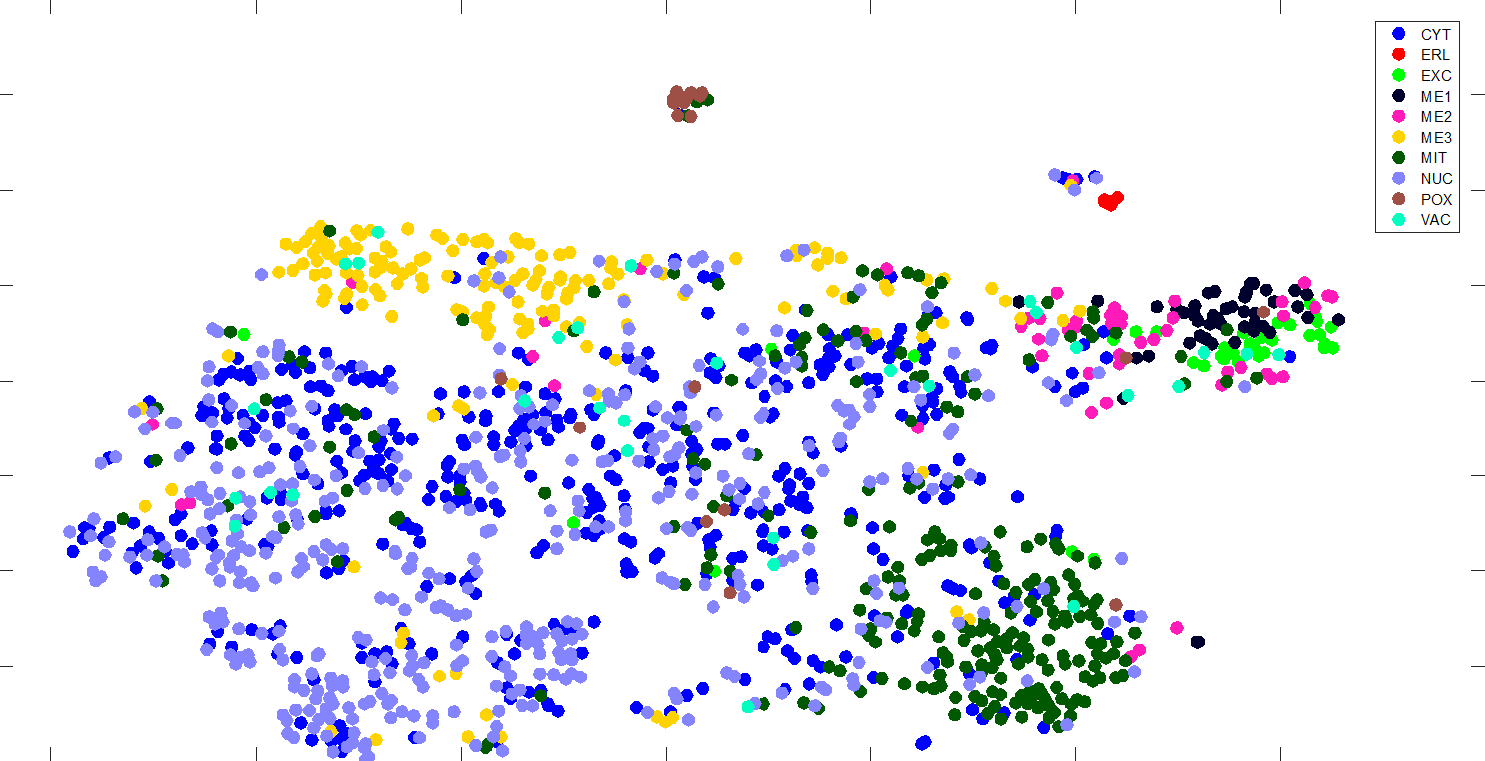
\includegraphics[width=0.9\linewidth]{figures/png/YeastTSNE}
	\caption[T-SNE visualization of Yeast dataset]{T-SNE visualization of Yeast dataset. Viewing in color is highly recommended.}
		\label{fig:yeasttsne}
\end{figure}



\paragraph{Cardiotocography Dataset}
Cardiotocography is the practice of monitoring fetal heartbeats during pregnancy.  The Cardiotocograph (CTG) is the machine used to monitor, and it produces cardiotocograms.    The dataset is based on \cite{ayres-de-campos_sisporto_2000} and was also used, in limited form, in \cite{ocak_medical_2013}, where the researchers achieved an impressive 100\% specificity (in this case, the correct classification of pathologic cardiotocograms).  Their sensitivity was also very high- 99.3\% on the training set.  Clearly here specificity is more important than sensitivity!  Unfortunately, these researchers left out approximately 200 samples of suspicious cardiotocograms, which confound things considerably.  There are good methodological reasons for doing this, of course- SVMs don't work as well with more than 2 classes, and culturally medicine is very concerned with sensitivity and specificity, which don't apply to non-binary problems in general.  We certainly aren't criticizing the good work medical researchers do, nor the lives they save.\\
We do include the suspect cardiotocograms, so we don't expect our results to be quite as clean. Further, there are two classification modes in this dataset, not 1.  The first is what we've mentioned already, the Normal, Suspect, Pathologic (NSP) classifications.  The second is the morphologic patterns 1-10.  These may or may not overlap with the NSP, but they provide a second way of looking at the data and evaluating it.  We have provided T-SNE visualizations with both colorings below in \ref{fig:cardio3tsne} and \ref{fig:cardio10tsne}.
\begin{figure}
	\centering
	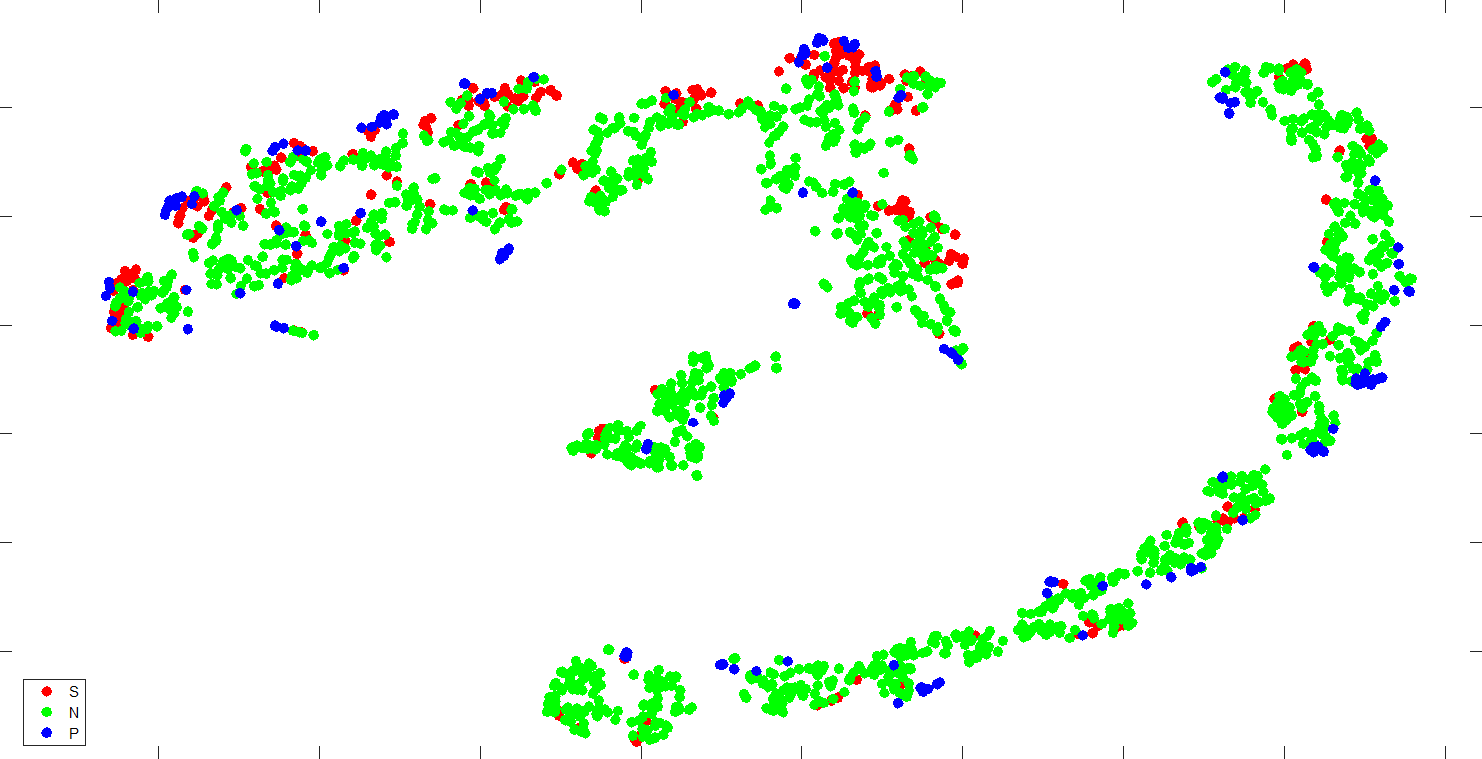
\includegraphics[width=0.9\linewidth]{figures/png/Cardio3TSNE}
	\caption[T-SNE visualization of Cardio dataset, NSP]{T-SNE visualization of Cardio dataset, following the NSP classification schema.}
	\label{fig:cardio3tsne}
\end{figure}
\begin{figure}
	\centering
	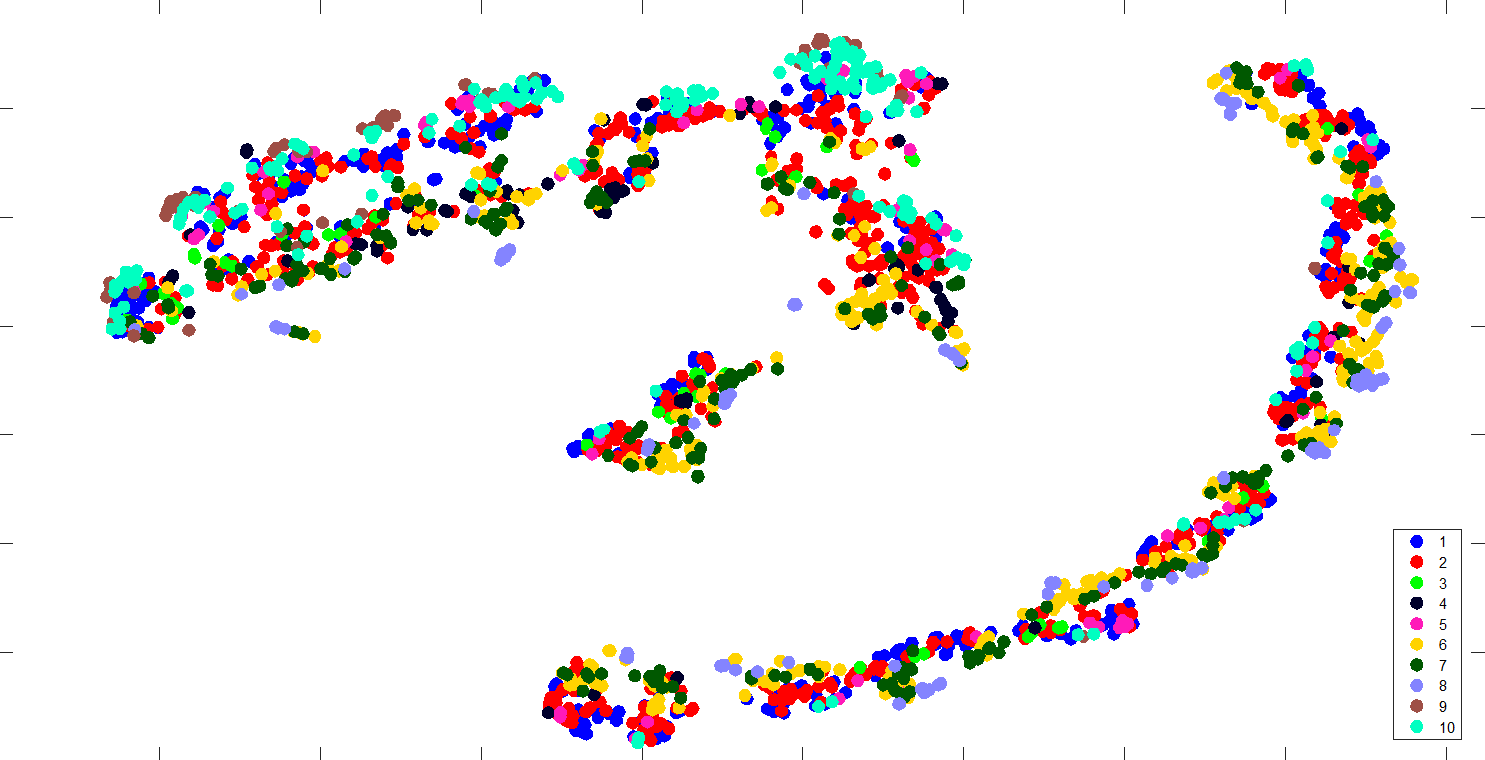
\includegraphics[width=0.9\linewidth]{figures/png/Cardio10TSNE}
	\caption[T-SNE visualization of Cardio dataset, morphology]{T-SNE visualization of Cardio dataset, following the 10-class morphology schema.  Viewing in color is highly recommended.}
	\label{fig:cardio10tsne}
\end{figure}
\paragraph{Bach's Chorales}
Bach composed all manner of music, but this dataset comprises 58 of his 4 part harmonies, called Chorales.  Originally made a dataset in \cite{radiocini} the music of 58 chorales are painstakingly broken into 5665 musical moments, such that every time there are 3 or more distinct notes being played it their proper key is classified- but there are confounding factors. Primarily, there might be added notes, which means a note must always be taken in context, which makes the problem much more difficult.  What was a fairly modest 36 classes (12 notes $\times$ 3 modes) becomes 108 when added notes are taken into account.  Originally the authors used a perceptron which scored 75\% accuracy, which is certainly much better than chance because, while there are 108 possible classes, only 102 can actually be found in the dataset.  \\We should note that we modified this dataset slightly.  Initially they were published in the order in which they occurred.  We added an additional feature including the key of the previous event and then randomized the order of the file before splitting it into training and testing sets.  The hopes were that our algorithms would be able to take advantage of the temporal information in their models, even if they weren't explicitly instructed that it was temporal.  The visualization (\ref{fig:bachtsne}) is difficult to read because of the many classes, but clearly delineates several inherent clusters.
\begin{figure}
	\centering
	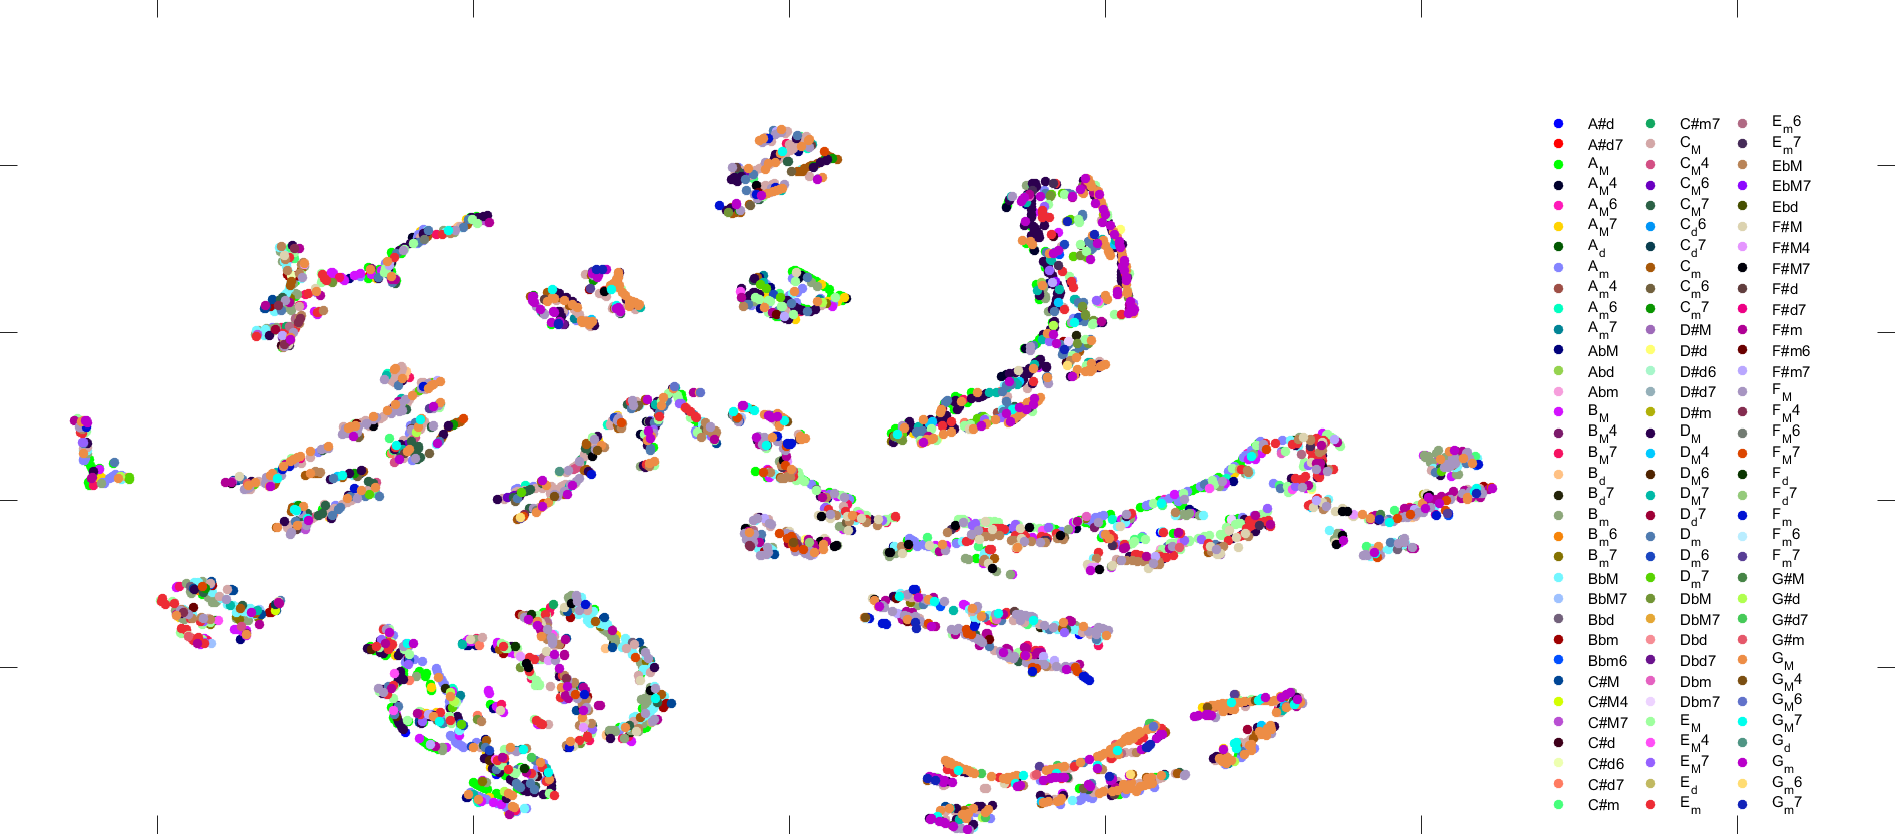
\includegraphics[width=0.9\linewidth]{figures/png/BachTSNE}
	\caption[T-SNE visualization of Bach dataset]{T-SNE visualization of 102 class Bach dataset.  Classes are incredibly difficult to distinguish, but instead focus on the overall shapes and distinct clusters.}
	\label{fig:bachtsne}
\end{figure}
\section{Results}
\subsection{Yeast}
\paragraph{CTree Baseline}:
0000000001111110000000\\
% TODO: interpret bits
As we can see, the baseline did fairly well regarding the 3 most common classes, but its ability to distinguish the less frequent classifications suffered giving it a final $\overline{A}$ of 64.1\%, or an overall accuracy of 74.6\%. \\
\begin{table}[h!]
\begin{tabular}{|c|c|c|c|c|c|c|c|c|c|c|c|}
\hline
Class&MIT&NUC&CYT&ME1&EXC&ME2&ME3&VAC&POX&ERL&Total
\\\hline
MIT&151&14&24&0&0&5&2&1&1&1&199\\
NUC&8&145&36&0&1&0&4&1&3&0&198\\
CYT&19&30&133&0&3&4&1&2&5&1&198\\
ME1&1&0&0&14&2&1&0&0&0&0&18\\
EXC&0&0&0&0&12&0&0&0&0&0&12\\
ME2&0&1&1&2&1&21&0&0&0&0&26\\
ME3&1&4&3&1&0&2&67&0&0&0&78\\
VAC&0&1&0&0&0&0&0&1&0&0&2\\
POX&0&0&1&0&0&0&0&0&5&0&6\\
ERL&0&0&0&0&0&0&0&0&0&3&3\\
\hline
Total:&180&195&198&17&19&33&74&5&14&5&740\\
TPR:&0.839&0.744&0.672&0.824&0.632&0.636&0.905&0.2&0.357&0.6&0.641\\
\hline
\end{tabular}
\caption[Yeast: Classification Tree without Feature Selection Confusion Matrix]{Classification Tree with all features included}
\label{tab:yeastctreebase}
\end{table}

\paragraph{CTree w/ feature selection}:
1111110001111100000000\\
% TODO:, interpret bits
With feature selection $\overline{A}$ increased modestly to 65.8\%, but accuracy declined to 68.4\%.\\
\begin{table}[h!]

\begin{tabular}{|c|c|c|c|c|c|c|c|c|c|c|c|}
	\hline
Class&MIT&NUC&CYT&ME1&EXC&ME2&ME3&VAC&POX&ERL&Total\\
MIT&131&13&9&0&0&1&2&0&2&0&158\\
NUC&8&87&26&0&1&0&1&2&0&0&125\\
CYT&33&87&158&0&3&2&4&2&4&0&293\\
ME1&1&0&0&13&2&1&0&0&0&0&17\\
EXC&1&0&0&1&11&1&0&0&0&0&14\\
ME2&5&2&1&2&2&26&0&0&0&1&39\\
ME3&1&5&3&1&0&2&67&0&0&0&79\\
VAC&0&1&0&0&0&0&0&1&0&0&2\\
POX&0&0&1&0&0&0&0&0&8&0&9\\
ERL&0&0&0&0&0&0&0&0&0&4&4\\
\hline
Total:&180&195&198&17&19&33&74&5&14&5&740\\
TPR:&0.728&0.446&0.798&0.765&0.579&0.788&0.905&0.2&0.571&0.8&0.658\\
\hline


\end{tabular}
\caption[Yeast:Classification Tree with Feature Selection Confusion Matrix]{Final Confusion Matrix: Classification Tree with feature selection}
\label{tab:yeastctreefeatures}
\end{table}

\paragraph{McNB Baseline}
000000001011000000000100010011001100110000\\
% TODO: , interpret bits
With all features, $\overline{A}$ was quite good: 85.9\%.  However, overall accuracy was 72.8\%.  
\\
\begin{table}[h!]
\begin{tabular}{|c|c|c|c|c|c|c|c|c|c|c|c|}
	\hline
Class&MIT&NUC&CYT&ME1&EXC&ME2&ME3&VAC&POX&ERL&Total\\
MIT&119&10&10&0&0&0&1&0&1&0&141\\
NUC&9&108&17&0&0&1&0&0&0&0&135\\
CYT&18&35&152&0&1&0&0&1&0&0&207\\
ME1&4&4&2&17&0&0&0&0&0&0&27\\
EXC&4&6&2&0&18&0&0&0&0&0&30\\
ME2&12&9&5&0&0&32&2&0&0&0&60\\
ME3&8&10&5&0&0&0&71&0&0&0&94\\
VAC&1&5&0&0&0&0&0&4&0&0&10\\
POX&5&8&5&0&0&0&0&0&13&0&31\\
ERL&0&0&0&0&0&0&0&0&0&5&5\\
\hline
Total:&180&195&198&17&19&33&74&5&14&5&740\\
TPR:&0.661&0.554&0.768&1&0.947&0.97&0.959&0.8&0.929&1&0.859\\
\hline
\end{tabular}
\caption[Yeast:Multiclass Na\"ive Bayes without Feature Selection Confusion Matrix]{Multiclass Na\"ive Bayes with all features included}
\label{tab:yeastmcnbbase}
\end{table}

\begin{table}[h!]
\paragraph{McNB w/ feature selection:}
111111101000010001001100011110110111110000
% TODO: Write writeup, interpret bits
With feature selection, Multiclass Na\"ive Bayes had the highest $\overline{A}$ of 87\%, though with an accuracy of only 72.8\%.  The disparity is accounted for in the accuracy across the first 3 classes, which make up more than $\frac{3}{4}$ of the dataset.  On them, accuracy ranged between abysmal and mediocre.  We can clearly see the danger of a highly skewed   
\\
\begin{tabular}{|c|c|c|c|c|c|c|c|c|c|c|c|}
	\hline
Class&MIT&NUC&CYT&ME1&EXC&ME2&ME3&VAC&POX&ERL&Total\\
\hline
MIT&124&22&17&0&0&0&0&0&1&0&164\\
NUC&8&90&21&0&0&0&0&0&0&0&119\\
CYT&13&36&134&0&1&0&0&0&0&0&184\\
ME1&3&1&1&17&0&0&0&0&0&0&22\\
EXC&2&3&1&0&18&0&0&0&0&0&24\\
ME2&9&8&4&0&0&33&0&0&0&0&54\\
ME3&15&20&12&0&0&0&74&0&0&0&121\\
VAC&2&9&3&0&0&0&0&5&0&0&19\\
POX&4&5&5&0&0&0&0&0&13&0&27\\
ERL&0&1&0&0&0&0&0&0&0&5&6\\
\hline
Total:&180&195&198&17&19&33&74&5&14&5&740\\
TPR:&0.689&0.462&0.677&1&0.947&1&1&1&0.929&1&0.87\\
\hline
\end{tabular}
\caption[Yeast: Multiclass Na\"ive Bayes with Feature Selection Confusion Matrix]{Final Confusion Matrix: Multiclass Na\"ive Bayes with feature selection included}
\label{tab:yeastmcnbfeatures}
\end{table}


\begin{table}[h!]
	\paragraph{Hunter:}
The Hunter underperformed the four other methods by any measure, and took a great deal (more than 100 times) more processor time to do it.  This was supposed to be the best case for the Hunters, and early indications say that it is.  $\overline{A}$ = .473\%, while accuracy is 51.1\%.  
\\
	% TODO: Write writeup, interpret bits
	\begin{tabular}{|c|c|c|c|c|c|c|c|c|c|c|c|}
		\hline
		Class&MIT&NUC&CYT&ME1&EXC&ME2&ME3&VAC&POX&ERL&Total\\
		\hline
MIT&105&17&12&0&0&0&0&0&0&0&134\\
NUC&2&37&10&1&0&1&3&0&0&0&54\\
CYT&43&94&142&0&5&3&2&1&10&0&300\\
ME1&4&1&0&8&1&3&7&0&0&0&24\\
EXC&9&2&3&0&9&7&0&0&2&0&32\\
ME2&1&9&6&6&4&12&1&1&0&2&42\\
ME3&14&5&11&2&0&6&58&1&0&0&97\\
VAC&2&28&13&0&0&1&3&2&0&0&49\\
POX&0&0&1&0&0&0&0&0&2&0&3\\
ERL&0&2&0&0&0&0&0&0&0&3&5\\
\hline
Total:&180&195&198&17&19&33&74&5&14&5&740\\
TPR:&0.583&0.19&0.717&0.471&0.474&0.364&0.784&0.4&0.143&0.6&0.473\\

		\hline
	\end{tabular}
	\caption[Yeast: Multiclass Na\"ive Bayes with Feature Selection Confusion Matrix]{Multiclass Na\"ive Bayes with feature selection included}
	\label{tab:yeasthunter}
\end{table}

Which classifier performed best is open for debate, both CTree and McNB are promising in their own ways.  CTree seems to do a better job with the bulk classes, and perhaps if you're optimizing average accuracy that's a good way to go- optimize a method for something it is less suited for, resulting in a kind of check on optimization gone awry.  Alternatively, maybe the status of the major classes don't particularly matter, and the focus instead is on discriminating between the outlier classes.  In that case, McNB clearly wins.  In any case, the Hunter performed.  It didn't do well, exactly, and with more time it might have done better, but that applies to any of these methods.  The difference is that the Hunter already had 10 times as many generations and still didn't manage to get anywhere even close to competitive.

\subsection{Cardiotocography NSP}
\paragraph{CTree Baseline}
\begin{table}[h!]
	\centering
	\begin{tabular}{|c|c|c|c|c|}
		\hline
		Class&Normal&Suspect&Pathologic&Total\\\hline
Normal&519&31&9&559\\
Suspect&12&408&0&420\\
Pathologic&10&0&74&84\\\hline
Total:&541&439&83&1063\\
TPR:&0.959&0.929&0.892&0.927\\
		\hline
	\end{tabular}
	\caption[CardioNSP: Classification Tree without Feature Selection Confusion Matrix]{Classification Tree without feature selection included}
	\label{tab:cardioNSPctreebase}
\end{table}
Accuracy: 94.1\%
\paragraph{CTree w/ Feature Selection}
\begin{table}[h!]
	\centering
	\begin{tabular}{|c|c|c|c|c|}
		\hline
		Class&Normal&Suspect&Pathologic&Total\\\hline
Normal&514&34&3&551\\
Suspect&12&405&0&417\\
Pathologic&15&0&80&95\\\hline
Total:&541&439&83&1063\\
TPR:&0.95&0.923&0.964&0.946\\

		\hline
	\end{tabular}
	\caption[CardioNSP: Classification Tree with Feature Selection Confusion Matrix]{Classification Tree with feature selection included}
	\label{tab:cardioNSPctree}
\end{table}
Accuracy: 93.9\%
\paragraph{McNB Baseline}
\begin{table}[h!]
	\centering
	\begin{tabular}{|c|c|c|c|c|}
		\hline
Class&Normal&Suspect&Pathologic&Total\\\hline
Normal&476&24&6&506\\
Suspect&37&408&2&447\\
Pathologic&28&7&75&110\\\hline
Total:&541&439&83&1063\\
TPR:&0.88&0.929&0.904&0.904\\
\hline
	\end{tabular}
	\caption[CardioNSP: Multiclass Na\"ive Bayes without Feature Selection Confusion Matrix]{Multiclass Na\"ive Bayes without feature selection included}
\label{tab:cardioNSPmcnbbase}
\end{table}
Accuracy 90.2\%
\paragraph{McNB w/ Feature Selection}
\begin{table}[h!]
	\centering
	\begin{tabular}{|c|c|c|c|c|}
		\hline
Class&Normal&Suspect&Pathologic&Total\\\hline
Normal&490&11&1&502\\
Suspect&28&427&0&455\\
Pathologic&23&1&82&106\\\hline
Total:&541&439&83&1063\\
TPR:&0.906&0.973&0.988&0.956\\
\hline
	\end{tabular}
	\caption[CardioNSP: Multiclass Na\"ive Bayes with Feature Selection Confusion Matrix]{Multiclass Na\"ive Bayes with feature selection included}
	\label{tab:cardioNSPmcnb}
\end{table}
Accuracy 94\%
\paragraph{Hunter}
\begin{table}[h!]
	\centering
	\begin{tabular}{|c|c|c|c|c|}
		\hline
		Class&Normal&Suspect&Pathologic&Total\\\hline
Normal&197&77&10&284\\
Suspect&183&322&4&509\\
Pathologic&161&40&69&270\\\hline
Total:&541&439&83&1063\\
TPR:&0.364&0.733&0.831&0.643\\
		\hline
	\end{tabular}
	\caption[CardioNSP: Hunter Confusion Matrix]{Hunter with feature selection included}
	\label{tab:cardioNSPHunter}
\end{table}
Accuracy 55\%
\subsection{Cardiotocography Morphology}
\paragraph{CTree Baseline}
\paragraph{CTree w/ Feature Selection}
\paragraph{McNB Baseline}
\paragraph{McNB w/ Feature Selection}
\paragraph{Hunter}

\subsection{Bach's Chorales}
\paragraph{CTree Baseline}
\paragraph{CTree w/ Feature Selection}
\paragraph{McNB Baseline}
\paragraph{McNB w/ Feature Selection}
\paragraph{Hunter}

\section{Final Thoughts}
It is clear that theoretically based algorithms are better at solving problems than trying to co-opt a GA to do it on its own.  
As for whether we should use McNB or CTree, the answer is clear: neither.  We've already written far better performing algorithms elsewhere, including aggregate trees and support vector machine optimizers.  The purpose of those algorithms was to give Hunters competition that wouldn't completely outclass them, and they failed in that regard.  This is at least partially because Na\"ive Bayes is such a robust first pass, and there are good reasons to use it in ensemble methods because it does such a good job extracting signal from messy data.\\
The most surprising performance was from CTree- while we have used trees in aggregate before, they performed far better alone than expected, in some regards holding their own up against Na\"ive Bayes, though mostly in terms of overall accuracy and only if we're being accommodating.  Still, their performance was better than we would have expected going into the project.\\
  